\documentclass[../main.tex]{subfiles}

\begin{document}

\section{Experiment}
\label{sec: Experiment}

\ref{sec: Human-Machine Ensemble Method} showed the number of humans that minimizes the expected squared error of the ensemble in the case where a machine and humans follow the proposed models.
However, it is unclear whether the proposed models is appropriate for real problems.
Furthermore, even if the proposed model is appropriate, it is impossible to know the true values of parameters $\varh$,$\covh$ and $\covmh$.
These can only be \emph{estimated} from past forecasts.
The distributions outputted by a machine $f_\theta(y|\x)$ are also based only on the training set, so they are not always adaptable to unknown inputs.
Therefore, we apply the proposed human-machine ensemble method to actual economic forecasts and investigate its performance by comparing with other forecasting methods.

In this chapter, Section~\ref{sub: Data} and Section~\ref{sub: Forecasting Models and Methodology} describe data and forecasting methods, respectively.
The results are in \ref{sec: Empirical Results}.

\subsection{Data}
\label{sub: Data}

We used inflation in the U.S. as targets of economic forecasts.
This section describes four inflation indicators and two surveys for economic forecasts.

\subsubsection{Inflation}

We consider four different measures of inflation: CPI-U for All Urban, All Items (\emph{CPI}); CPI-U for All Urban, All items less food and energy (\emph{CoreCPI}); Personal Consumption Expenditures (\emph{PCE}); and PCE excluding food and energy (\emph{CorePCE}).
All measures are seasonally adjusted.
CPI and CoreCPI are obtained from the Bureau of Labor Statistics\footnote{\url{https://www.bls.gov/}} and the sample period is from Jan.\ 1957 to Oct.\ 2016.
PCE and CorePCE are obtained from the Bureau of Economic Analysis\footnote{\url{https://www.bea.gov/}} and the sample period is from Jan.\ 1959 to Oct.\ 2016.

CPI measures the total cost of goods and services purchased by urban consumers.
It is commonly used as an indicator of inflation.
CoreCPI excludes food and energy price from CPI\@.
Short-term fluctuations of CoreCPI is smaller than CPI because the prices of food and energy change easily.

PCE also measures the cost of goods and services purchased by consumers, but includes costs that CPI does not include such as medical expenses, and the data source is different.
In addition, calculation procedures are different such that PCE uses chained weights while CPI uses fixed weights.
CorePCE exclude food and energy price from PCE\@.

\begin{figure}
  \centering
  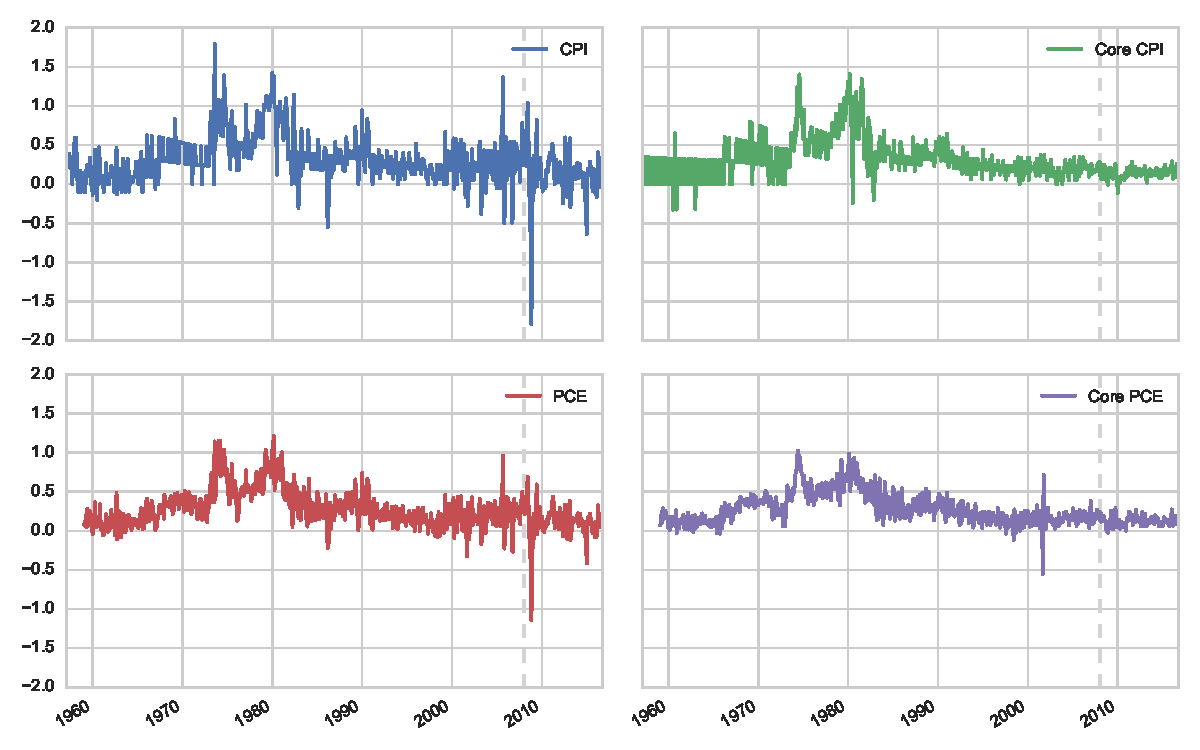
\includegraphics[width=\textwidth]{experiment-series.pdf}
  \caption{
    Monthly inflation rate measured by CPI, CoreCPI, PCE, and CorePCE\@.
    The dotted line represents 2008, which is the boundary between the traing set and test set.
  }\label{fig: series}
\end{figure}

This thesis defines inflation rate from $t - 1$ to $t$ as:
\begin{equation}
  \pi_t = \log \left(\frac{P_t}{P_{t-1}}\right) \times 100,
  \label{eq: inflation}
\end{equation}
where $P_t$ is the level of an index at time $t$.
This thesis uses the terms ``inflation'' and ``inflation rate'' as defined in (\ref{eq: inflation}).
$\pi_t$ can be regarded as an approximation of the normal change rate by the following first order Taylor expansion approximation, assuming that the change is sufficiently small,
\begin{equation*}
  \log \left(\frac{P_t}{P_{t-1}}\right) = \log \left(1 + \frac{P_t - P_{t - 1}}{P_{t - 1}}\right) \approx \frac{P_t - P_{t - 1}}{P_{t - 1}}.
\end{equation*}
Figure~\ref{fig: series} shows monthly inflation of the four indices.

\subsubsection{Surveys}
\label{ssub: Surveys}

We used two surveys for economic forecasts: the Livingston Survey%
\footnote{\url{https://www.philadelphiafed.org/research-and-data/real-time-center/livingston-survey}} and the Survey of Professional Forecasters%
\footnote{\url{https://www.philadelphiafed.org/research-and-data/real-time-center/survey-of-professional-forecasters/}} (SPF) as forecasts by humans.
The Federal Reserve Bank of Philadelphia has been taking these surveys to economic experts.
While the Livingston Survey includes the economists from government and academia, the SPF mainly covers industry.
Figure~\ref{fig: survey forecasts} shows forecasts by each survey.

\begin{figure}
  \centering
  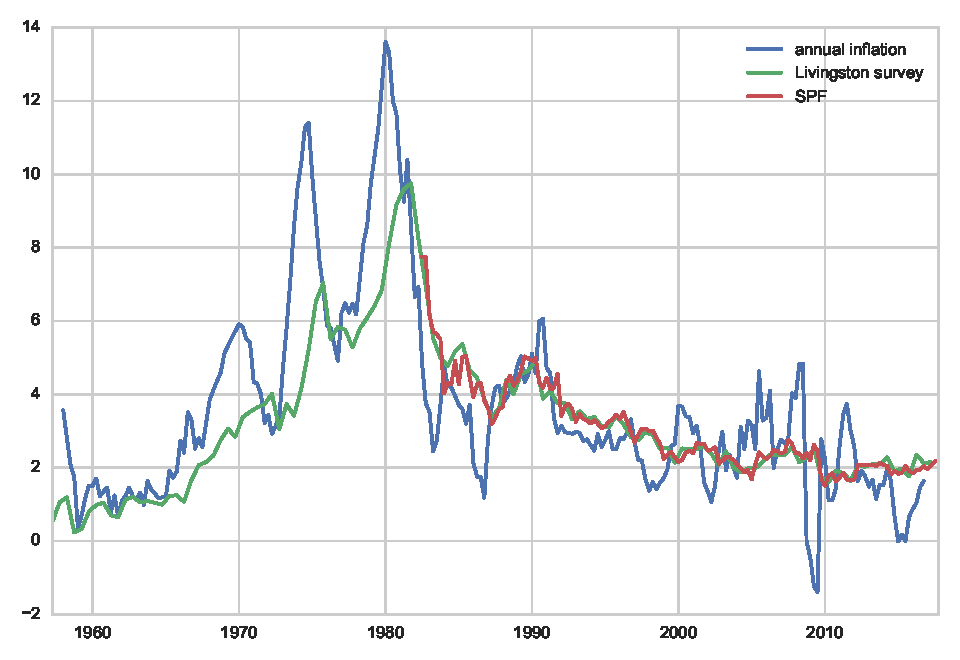
\includegraphics[width=\textwidth]{experiment-surveys.pdf}
  \caption{
    Annual CPI change rate and averaged forecasts by the Livingston Survey and the SPF\@.
  }\label{fig: survey forecasts}
\end{figure}

\paragraph{Livingston Survey}

The Livingston Survey is conducted twice a year, in June and in December, from 1946.
This study treats from Jun.\ 1957 to Jun.\ 2016.
The Livingston Survey includes only CPI as a survey item.
It was reorganized in 2004, and started to forecast seasonally adjusted series from not seasonally adjusted series.
It forecasts inflation 6 months later and 12 months later as the short term forecasts.
The average number of respondents to 12 months forecast was $45.6$ and the standard deviation was $11.6$.

\paragraph{SPF}

The SPF began in 1968 and is conducted quarterly.  It covers all four indicators as survey items.
However, the survey of CPI started in 1981Q3, and the other three indicators started in 2007Q1.
In this thesis, we used all the survey data up to 2015Q4.
The average number of respondents to CPI was $34.4$ and the standard deviation was $9.3$.

\subsection{Forecasting Models and Methodology}
\label{sub: Forecasting Models and Methodology}

This section describes four forecasting methods and evaluation method for the experiment.
The forecasting methods are a time-series model \emph{ARMA(1,1)} as benchmark, a \emph{recurrent neural networks (RNN)} as machine forecasts, survey forecasts as human forecasts, and the human-machine ensemble method proposed in \ref{sec: Human-Machine Ensemble Method}.
We created models that predict annual change rate of the four indices using ARMA(1,1) and RNN, and also created models that predict 6 months change rate of CPI\@.
Due to the restrictions on the survey data, 12 months and 6 months forecasts for CPI are made from the Livingston Survey, and annual forecasts for all indices are made from the SPF\@.
The human-machine ensemble method follows the restrictions of surveys.
The data set is divided into the training set and test set, and creation of prediction models does not include the test set.
Forecasting accuracy is evaluated by \emph{Root Mean Squared Error (RMSE)} for the test set.

\subsubsection{Time-series model}
\label{ssub: Time-series model}

We used an \emph{autoregressive moving average (ARMA) model} for benchmark forecasts as well as Ang et al.~\cite{Ang2007}.
ARMA(1,1) is a traditional model for inflation forecasts.
Ang et al.\ made a model based on quarterly inflation rate, and we also did so.

Assume that inflation is stationary to apply an ARMA model.
A process is stationary means that the following equations hold for arbitrary $t$ and $k$:
\begin{align}
  \begin{split}
    E[\pi_t] &= \mu \\
    \cov(\pi_t, \pi_{t-k}) &= E[(y_t - \mu)(y_{t-k} - \mu)] = \lambda_k,
  \end{split}
\end{align}
where $\mu$ and $\lambda_k$ are constants.
This assumption is totally different from the model of \ref{sec: Human-Machine Ensemble Method}, which assumed that the expected error varies depending on the situation $t$.

The specifications of the ARMA(1,1) model is
\begin{equation}
  \pi_{t + 1} = \mu + \phi\pi_t + \psi\epsilon_t + \epsilon_{t + 1},
\end{equation}
where $\epsilon_t$ is white noise with variance $\sigma^2$~\cite{沖本2010}.
The parameters are $\mu$, $\phi$, $\psi$, $\sigma^2$, and they are estimated by maximum likelihood conditional on a zero initial residual, assumed the Gaussian white noise.

Applying this model, when an inflation rate at time $t$, $\pi_{t}$, is given, the forecast value of inflation rate after one period is
\begin{equation}
  \hat{\pi}_{t+1|t} = E[\pi_{t + 1}|\pi_t] = \mu + \phi\pi_t + \psi\hat{\epsilon}_t.
\end{equation}
$\hat{\epsilon}_t$ is obtained by sequentially approximating like $\hat{\epsilon}_2 = \pi_2 - \mu - \phi\pi_1, \hat{\epsilon_3} = \pi_3 - \mu - \phi\pi_2 - \psi\hat{\epsilon_2}, \dots$, in which the initial value is $\hat{\epsilon}_0 = 0$.
Since the term of $\epsilon$ disappears from forecasts after two period, the forecast values can be obtained sequentially by the following relationship:
\begin{equation*}
  \hat{\pi}_{t + k|t} = \mu + \phi\hat{\pi}_{t + k - 1|t}.
\end{equation*}
However, $\hat{\pi}_{t + k}$ is a change rate for one period from $t+k-1$ to $t+k$, so the change rate from $t$ to $t+k$ is the sum of $k$ periods:
\begin{equation}
  \hat{\pi}_{t + k, k} = \sum_{i=1}^k \hat{\pi}_{t+i}.
\end{equation}
When $k = 2$, it is the 6 months later forecast, and when $k = 4$, it is the 12 months later forecast.

When using ARMA(1,1), the expected squared error of a forecast of one period ahead is always $\sigma^2$ regardless of $t$.
Therefore, it is not applicable to the machine model in Section~\ref{ssub: Machine model}, which assumed the expected error varies depending on the situation.
The next section describes RNN that can be used as a machine model for the proposed human-machine ensemble method.

\subsubsection{Recurrent neural network model}
\label{ssub: Recurrent neural network model}

\begin{figure}
  \centering
  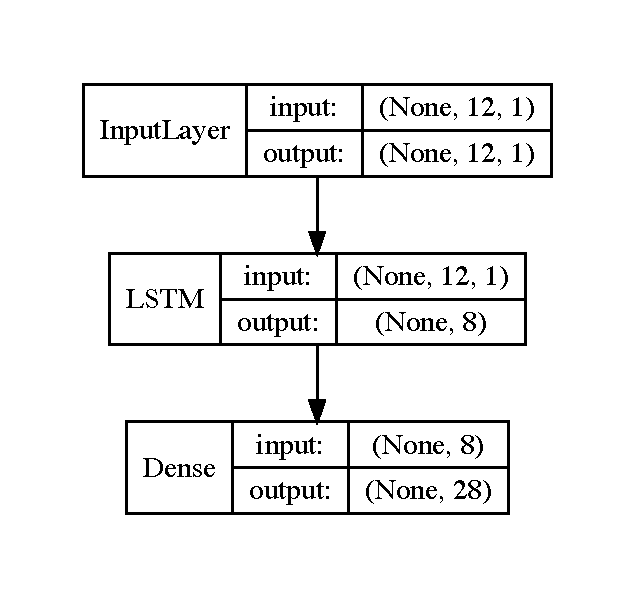
\includegraphics[width=0.6\textwidth]{experiment-machine_model.pdf}
  \caption{
    The RNN architecture used in the experiment.
    The inside of parentheses describes the dimentions of data, and the first term represents the batch size 32 instead of ``None.''
    The output dimention 28 is for forecasts of annual CPI change rate.
  }\label{fig: RNN architecture}
\end{figure}

We used a RNN model that includes \emph{Long short-term memory} (LSTM) units in a hidden layer.
Let $\theta$ denote the RNN model, which outputs discrete probability distributions $f_\theta(y|\x)$ when the past 12 months inflation $\x = [\pi_{t-11}, \pi_{t-10}, \dots, \pi_t]$ are given.
The forecast value $y$ is an inflation rate for 6 months $\hat{\pi}_{t+6,6}$ or an inflation rate for 12 months $\hat{\pi}_{t+12,12}$.
Figure~\ref{fig: RNN architecture} shows the RNN architecture that realizes these input and output.
By using this architecture, we created five models that forecast annual inflation rates of the four indices, and CPI change rate for 6 months.
The rest of this section describes the details of the architecture and how to create the prediction models.

\paragraph{LSTM}

\begin{figure}
  \centering
  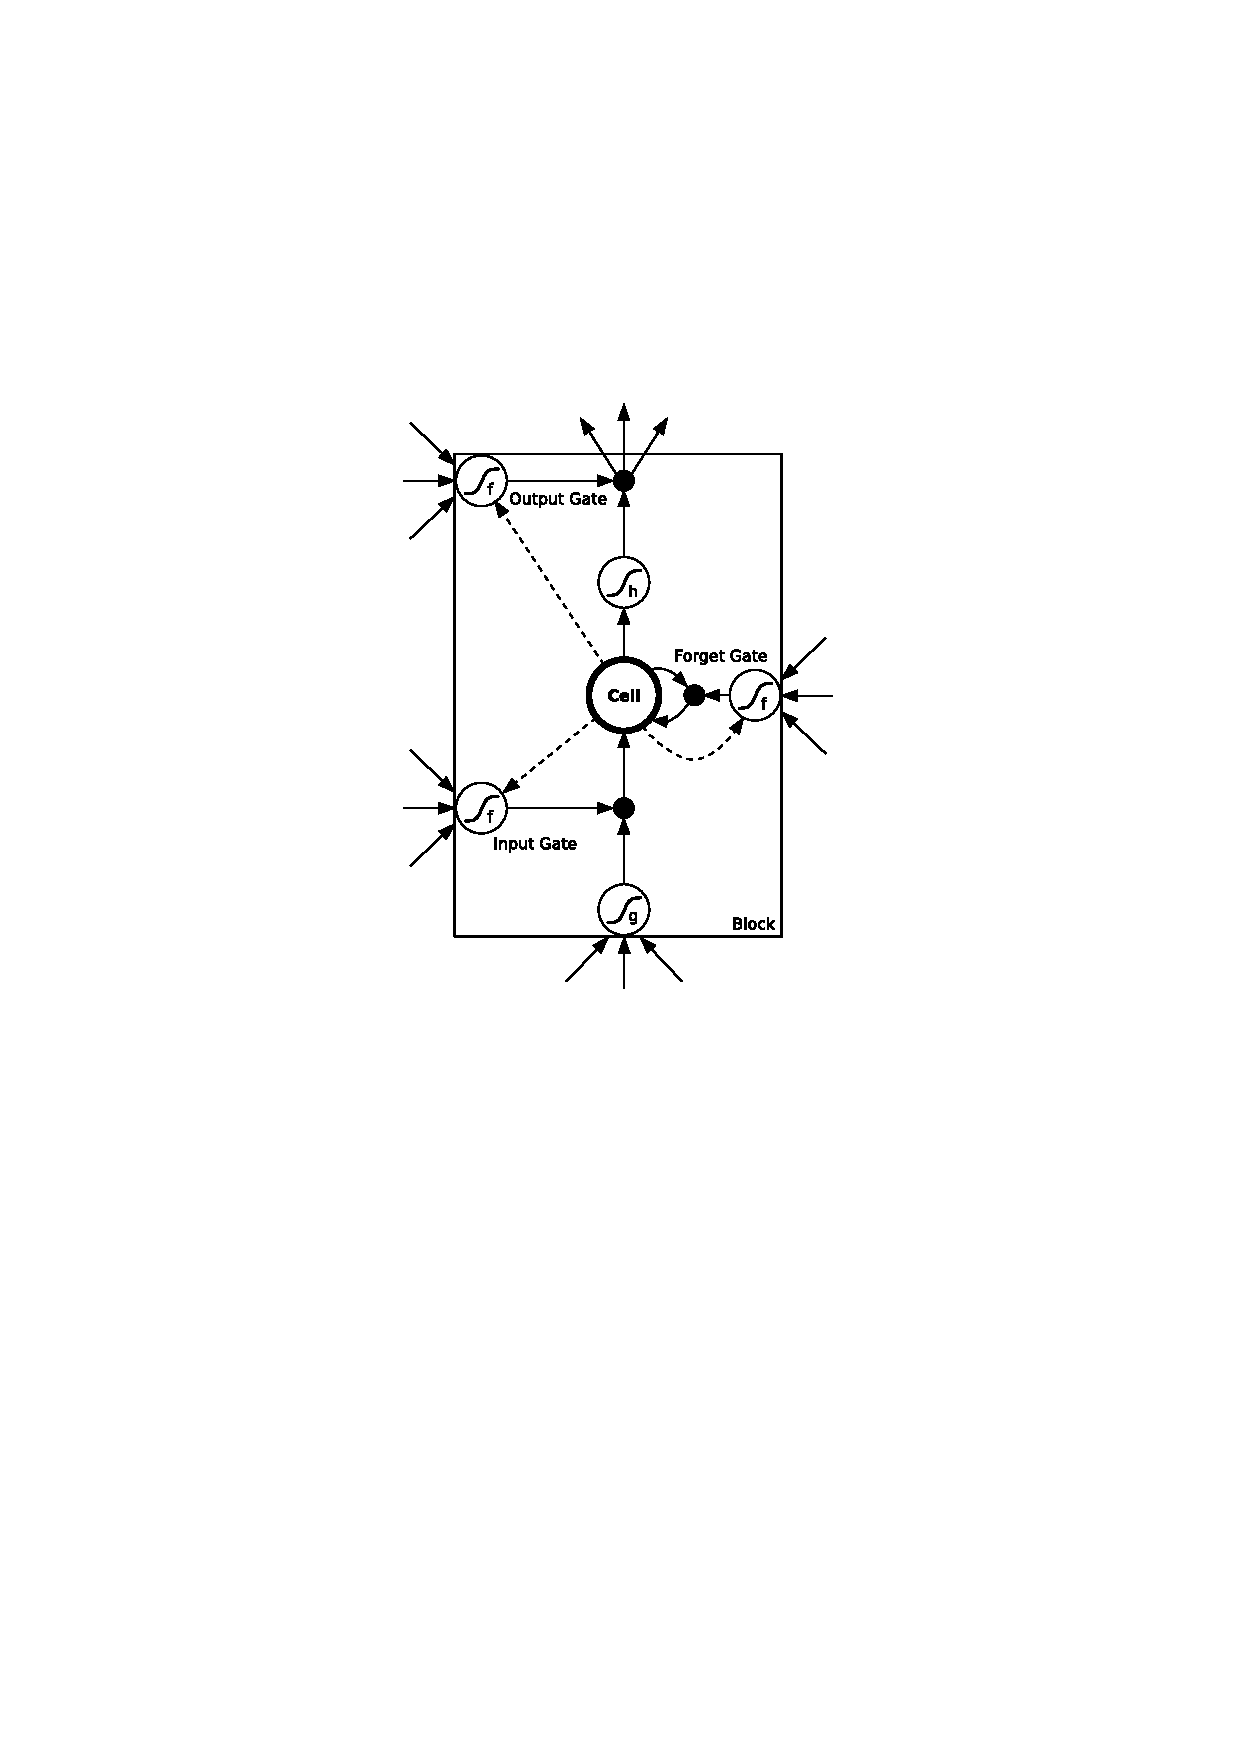
\includegraphics[width=0.5\textwidth]{experiment-lstm.pdf}
  \caption{
    LSTM memory block~\cite{Graves2012}
  }\label{fig: LSTM}
\end{figure}

Ordinary RNN has a problem that, given a long input sequence, the gradient rapidly increases or disappears when backpropagation is applied.
It is called \emph{vanishing gradient problem}.
The LSTM deals with this problem, and makes long-term memory possible~\cite{Graves2012, 岡谷2015}.
Replace units in each hidden layer of a basic RNN with LSTM memory blocks shown in Figure~\ref{fig: LSTM}.
It looks like there are four inputs, but they are all the same, and identical to the input of a unit in an ordinary RNN's hidden layer.
In the center of the block is a cell.
Small black circles around the cell are gates, which have activation function $f$.
As logistic sigmoid is usually used for $f$, the gate activations are between 0 (gate close) and 1 (gate open).
The cell stores a state, and realizes the memory by inputting the state to itself after one time interval.
However, a forget gate is on the way, and if the activation is close to 0, the state will be forgotten.
The outputs of activation functions $g$ and $h$ at the cell input and output are also transmitted if the activation of the gate is close to 1, and are blocked if it is close to 0.
With the above mechanism, the LSTM overcomes the limitation of RNN\@.
The experiment used eight LSTM units in the hidden layer, with $\tanh$ for the activation functions $g$ and $h$.

\paragraph{Output layer}

\begin{table}
  \caption{
    The minimum value, maximum value, number of output labels and difference between labels in each index.
  }\label{tab: output label}
  \begin{center}
    \begin{tabular}{lrrrrr}
\toprule
{} &  CPI(12M) &  CPI(6M) &  CoreCPI &   PCE &  CorePCE \\
\midrule
min  &       0.1 &     -0.4 &       0.7 &   0.5 &       0.9 \\
max  &      13.6 &      7.4 &      12.7 &  11.0 &       9.9 \\
size &        28 &       27 &        25 &    22 &        19 \\
step &       0.5 &      0.3 &       0.5 &   0.5 &       0.5 \\
\bottomrule
\end{tabular}

  \end{center}
\end{table}

As mentioned in Section~\ref{ssub: Machine model}, the activation function of the output layer uses the \emph{softmax function} so that the prediction model can output probability distributions.
Let $u_k$ denote input of unit $k$, and let $o_k$ denote output.
Then, the softmax function is
\begin{equation}
  o_k = \frac{\exp(u_k)}{\sum_{j=1}^K\exp(u_j)},
\end{equation}
where $K$ is the number of units in the output layer.
The sum of outputs $v_1, \dots, v_K$ is always $1$.
And the output $o_k$ can be interpreted as the probability of belonging to the corresponding class.
Making the labels $y_1, \dots, y_K$ correspond to each unit of the output layer realizes the output of discrete probability distributions.
For the labels, separate every 0.5 from the minimum value to the maximum value in the target outputs of training set.
For example, when forecasting the annual CPI change rate, since the minimum value and the maximum value in the training set are $0.13$ and $13.62$ respectively, the values of labels are $[0.1, 0.6, 1.1, \dots, 13.6]$, and the number of units is $K = 28$.
Table~\ref{tab: output label} shows the minimum and maximum values, the number of labels, and the difference between labels in each series.
Only when forecasting the 6 months CPI change rate, we set the step as $0.3$ to make the dimensions of the outputs similar to others.

\paragraph{Training}

We divided the data set into the training set and test set.
Creation of models uses only training set.
The test set is for evaluation.
The pairs of input and output are prepared as follows:
First, the input is a sequence of monthly inflation for the past 12 months $\x_t = [\pi_{t-11}, \dots, \pi_t]$ from a time $t$.
And these are normalized with the maximum value in the training set as 1.
On the other hand, the output is a vector that has $K$ elements $\bm{d}_t = [0, 0, \dots, 1, \dots, 0]$, where the $k$th value is 1 and the others are 0 because $y_k$ is closest to the correct value.
Furthermore, we used the \emph{cross entropy} as the error function:
\begin{equation}
  E(\bm{w}) = - \sum_{t=1}^T\sum_{k=1}^K d_{tk}\log v_k(\x_t;\bm{w}).
\end{equation}
The cross entropy is obtained by inverting the log-likelihood of parameters $\bm{w}$ for the training set $\{(\x_t, \bm{d}_t)\}(t = 1,\dots,T)$, when assumed the output is posterior distribution.
We used the \emph{RMSprop} for the learning algorithm, and set the batch size 32.
We stopped learning after 400 epochs, which number is obtained by cross validation.

\subsubsection{Survey forecasts}

In the Livingston Survey and the SPF, the number of respondents is different for every survey.
The minimum number of respondents through the both surveys is 9.
Armstrong~\cite{Armstrong2001} has proposed the principles for combining forecasts, and one of them is ``use at least five forecasts when possible.''
Hence, we sampled five forecasters randomly from each survey to make the number of forecasters equal.
The average values are regarded as the forecasts of the survey.

In addition, it is necessary to convert the surveyed values to appropriate inflation rate.
The rest of this section describes the methods to calculate the forecast values based on the documentation of each survey.

\paragraph{Livingston Survey}

The participants in the Livingston Survey respond with not inflation rate but CPI level.
The Livingston Survey presents the index level 2 months before to the participants.
Based on that level, the participants forecast the value of the current month, $\hat{P}_t$, the one of 6 months after, $\hat{P}_{t+6}$, and the one of 12 months after, $\hat{P}_{t+12}$.
However, it was in 1992 that the survey began to include the forecasts of the current month.
According to the presence or absence of the forecast value of the current month, the forecast value of $m$ months after, $\hat{\pi}_{t+m, m}$, is calculated by
\begin{equation}
  \hat{\pi}_{t+m, m} =
    \begin{cases}
      \log\left(\frac{\hat{P}_{t+m}}{\hat{P}_t}\right) & (\text{if } \hat{P}_t \text{ exists}) \\
      \log{\left(\frac{\hat{P}_{t+m}}{P_{t-2}}\right)}^{\frac{m}{m+2}} & (\text{otherwise}).9
    \end{cases}
\end{equation}

\paragraph{SPF}

The participants in the SPF respond with inflation rate, but this is a simple change rate $P_{t+12}/P_t -1$, not based on the definition of equation (\ref{eq: inflation}).
It is impossible to convert this value to the inflation rate of (\ref{eq: inflation}), so the experiment regards it as the approximation.
Note that since the forecast values are biased somewhat higher by not taking logarithm, the error becomes slightly larger.

\subsubsection{Human-machine ensemble}

The Human-machine ensemble method combines the RNN models and individual forecasts from each survey.
There are the five RNN models, which forecast annual inflation rate of CPI after 6 months and CPI, CoreCPI, PCE, and CorePCE after 12 months.
The Livingston Survey forecasts the index level of CPI after 6 months and 12 months, and the SPF forecasts annual inflation of the four indices.

Execution of the human-machine ensemble method requires the three parameters, $\varh$, $\covh$ and $\covmh$.
We estimated these parameters from the forecasts for the training set.
Let $N$ denote the number of participants in the training set, and let $\varepsilon_{h_i}$ and $\var(\varepsilon_{h_i})$ denote the error and the variance of a participant $i$ respectively.
Then, $\varh$ is estimated by
\begin{equation}
  \varh = \frac{1}{N}\sum_{i=1}^N\var(\varepsilon_{h_i}).
\end{equation}
Also, $\covh$ and $\covmh$ is estimated by equations (\ref{eq: covh}) and (\ref{eq: covmh}) using the unbiased covariance for $\cov(\varepsilon_{h_i}, \varepsilon_{h_j})$.

Section~\ref{ssub: Theroretical results} describes the optimal number of humans does not always exist.
However, in reality there is an upper limit $N_{\max}$ depending on the number of respondents.
Therefore, for the human-machine ensemble method, we used the $n$ that minimizes the expected error in the range of $0 \leq n \leq N_{\max}$.
In this case, unless $\MSE(Y_{\theta, h}(0)) = \MSE(Y_{\theta, h}(N_{\max}))$ holds, $n$ is specified uniquely.
When this equation holds, we set $n^\ast = N_{\max}$.
The experiment fixed $N_{\max} = 5$, which is the same as the members sampled in the survey forecasts.
Furthermore, when the expected error of humans only is less than that of combination of humans and a machine, the ensemble does not include the machine forecast.

\subsubsection{Assessing forecasting methods}
\label{ssub: Assessing forecasting methods}

The test set starts from 2008.
We also prepared the test set that starts from 1998 only for CPI\@.
The reason is that the SPF has the short sample period since it started from 1981 and the Livingston Survey forecasts only CPI\@.

The creation of RNN models and estimation of the ensemble parameters uses only the training set.
The ARMA(1,1) model is recreated at each forecasting since the creation of the model is easier than RNN\@.
That is, when forecasting annual inflation at 2008Q1, the creation of the model uses the samples up to 2007Q1, and when forecasting it at 2008Q2, the model is recreated using the samples up to 2007Q2.
Thus, the creation of ARMA(1,1) models uses the data up to the time of forecasting.

The frequency of forecasts in the test set is quarterly as the same to the benchmark, ARMA(1,1).
The number of samples in the test set that starts 2008 is $35$ from 2008Q1 to 2016Q3.
The Livingston Survey and the ensemble using it can only make forecasts on June and December, so the number of samples in the test set that starts 2008 is $17$, and the one that starts 1998 is $37$.
Although the RNN models can make forecasts monthly, they forecast only on March, June, September and December.

\begin{table}
  \caption{
    The varieties of the ensembles.
  }\label{tab: varieties of ensemble}
  \begin{center}
    \footnotesize
    \begin{tabular}{llllllll}
\toprule
{} & CPI-LIV & CPI-SPF &   CoreCPI &   PCE &   CorePCE & CPI-6M & CPI-1998 \\
\midrule
target index   &     CPI &     CPI &  CoreCPI &   PCE &  CorePCE &    CPI &      CPI \\
survey source   &     LIV &     SPF &       SPF &   SPF &       SPF &    LIV &      LIV \\
forecast period &     12M &     12M &       12M &   12M &       12M &     6M &      12M \\
dataset boundary &    2008 &    2008 &      2008 &  2008 &      2008 &   2008 &     1998 \\
\bottomrule
\end{tabular}

  \end{center}
\end{table}

Table~\ref{tab: varieties of ensemble} shows the all ensembles.
There are seven different ensembles depending on the target index, the survey source, the period to forecast, and the boundary of the training and test set.

We assess forecast accuracy with the \emph{Root Mean Squared Error (RMSE)}.
When an actual inflation and forecast value at time $t$ is $y_i$ and $\hat{y}_i$ respectively, and forecasting $M$ times, the RMSE is
\begin{equation}
  \RMSE(\bm{\hat{y}}) = \sqrt{\frac{1}{M}\sum_{i=1}^{M}(y_i - \hat{y}_i)}.
\end{equation}
In addition, we also report the ratio of RMSEs relative to the benchmark, ARMA(1,1).

\end{document}
